%\VignetteIndexEntry{Introduction to the dataRetrieval package}
%\VignetteDepends{}
%\VignetteSuggests{}
%\VignetteImports{}
%\VignettePackage{}

\documentclass[a4paper,11pt]{article}

\usepackage{amsmath}
\usepackage{times}
\usepackage{hyperref}
\usepackage[numbers, round]{natbib}
\usepackage[american]{babel}
\usepackage{authblk}
\usepackage{footnote}
\usepackage{placeins}
\renewcommand\Affilfont{\itshape\small}
\usepackage{Sweave}
\renewcommand{\topfraction}{0.85}
\renewcommand{\textfraction}{0.1}
\usepackage{graphicx}


\textwidth=6.2in
\textheight=8.5in
\parskip=.3cm
\oddsidemargin=.1in
\evensidemargin=.1in
\headheight=-.3in

%------------------------------------------------------------
% newcommand
%------------------------------------------------------------
\newcommand{\scscst}{\scriptscriptstyle}
\newcommand{\scst}{\scriptstyle}
\newcommand{\Robject}[1]{{\texttt{#1}}}
\newcommand{\Rfunction}[1]{{\texttt{#1}}}
\newcommand{\Rclass}[1]{\textit{#1}}
\newcommand{\Rpackage}[1]{\textit{#1}}
\newcommand{\Rexpression}[1]{\texttt{#1}}
\newcommand{\Rmethod}[1]{{\texttt{#1}}}
\newcommand{\Rfunarg}[1]{{\texttt{#1}}}

\begin{document}
\Sconcordance{concordance:dataRetrieval.tex:dataRetrieval.Rnw:%
1 126 1 49 0 1 7 15 1 1 14 55 1 3 0 36 1 2 0 11 1 24 %
0 24 1 3 0 23 1 3 0 6 1 7 0 18 1 3 0 25 1 1 0 17 1 9 %
0 6 1 7 0 21 1 8 0 16 1 2 0 11 1 23 0 21 1 9 0 20 1 3 %
0 6 1 17 0 27 1 6 0 11 1 9 0 15 1 20 0 21 1 4 0 21 1 %
4 0 17 1 7 0 22 1 8 0 19 1 4 0 9 1 4 0 78 1 1 2 9 1 1 %
4 4 1 20 0 44 1 4 0 32 1 4 0 21 1 4 0 21 1 37 0 13 1 %
9 0 95 1 4 0 9 1 12 0 13 1 4 0 14 1 4 0 5 1 4 0 23 1 %
18 0 8 1 4 0 55 1}


%------------------------------------------------------------
\title{The dataRetrieval R package}
%------------------------------------------------------------
\author[1]{Laura De Cicco}
\author[1]{Robert Hirsch}
\affil[1]{United States Geological Survey}



\maketitle
\tableofcontents

%------------------------------------------------------------
\section{Introduction to dataRetrieval}
%------------------------------------------------------------ 
The dataRetrieval package was created to simplify the process of getting hydrologic data in the R enviornment. It has been specifically designed to work seamlessly with the EGRET R package: Exploration and Graphics for RivEr Trends (EGRET). See: \url{https://github.com/USGS-R/EGRET/wiki} for information on EGRET. EGRET is designed to provide analysis of water quality data sets using the WRTDS method of data analysis (WRTDS is Weighted Regressions on Time, Discharge and Season) as well as analysis of streamflow trends using robust time-series smoothing techniques.  Both of these capabilities provide both tabular and graphical analyses of long-term data sets.


The dataRetrieval package is designed to retrieve many of the major data types of USGS hydrologic data that are available on the web, but also allows users to make use of other data that they supply from spreadsheets.  Section 2 provides examples of how one can obtain raw data from USGS sources on the web and ingest them into data frames within the R environment.  The functionality described in section 2 is for general use and is not tailored for the specific uses of the EGRET package.  The functionality described in section 3 is tailored specifically to obtaining input from the web and structuring them specifically for use in the EGRET package.  The functionality described in section 4 is for converting hydrologic data from user-supplied spreadsheets and structuring them specifically for use in the EGRET package.

For information on getting started in R and installing the package, see Appendix (\ref{sec:appendix1}): Getting Started.


%------------------------------------------------------------
\section{General USGS Web Retrievals}
%------------------------------------------------------------ 
In this section, we will run through 5 examples, documenting how to get raw data from the web. This includes site information (\ref{sec:usgsSite}), measured parameter information (\ref{sec:usgsParams}), historical daily values(\ref{sec:usgsDaily}), real-time (unit) values (\ref{sec:usgsRT}), and water quality data (\ref{sec:usgsWQP}) or (\ref{sec:usgsSTORET}). We will use the Choptank River near Greensboro, MD as an example.  The site-ID for this gage station is 01491000. Daily discharge measurements are available as far back as 1948.  Additionally, forms of nitrate have been measured dating back to 1964. The functions/examples in this section are for raw data retrieval.  This may or may not be the easiest data to work with.  In the next section, we will use functions that retrieve and process the data in a dataframe that may prove more friendly for R analysis.

%------------------------------------------------------------
\subsection{Introduction}
%------------------------------------------------------------
The United States Geological Survey organizes their hydrological data in standard structure.  Streamgages are located throughout the United States, and each streamgage has a unique ID.  Often (but not always), these ID's are 8 digits.  The first step to finding data is discoving this 8-digit ID. One potential tool for discovering data is Environmental Data Discovery and Transformation (EnDDaT): \url{http://cida.usgs.gov/enddat/}.  Follow the example on the EnDDaT web page to learn how to discover USGS stations and available data from any location in the United States. 

Once the site-ID is known, the next required input for USGS data retrievals is the 'parameter code'.  This is a 5-digit code that specifies what measured paramater is being requested.  A complete list of possible USGS parameter codes can be found at:

\url{http://nwis.waterdata.usgs.gov/usa/nwis/pmcodes?radio_pm_search=param_group&pm_group=All+--+include+all+parameter+groups&pm_search=&casrn_search=&srsname_search=&format=html_table&show=parameter_group_nm&show=parameter_nm&show=casrn&show=srsname&show=parameter_units}

Not every station will measure all parameters. A short list of commonly measured parameters is shown in Table \ref{tab:params}.



% latex table generated in R 3.0.0 by xtable 1.7-1 package
% Mon Apr 08 10:09:40 2013
\begin{table}[!ht]
\centering
\caption{Common USGS Parameter Codes} 
\label{tab:params}
\begin{tabular}{ll}
  \hline
pCode & shortName \\ 
  \hline
00060 & Discharge [cfs] \\ 
  00065 & Gage height [ft] \\ 
  00010 & Temperature [C] \\ 
  00045 & Precipitation [in] \\ 
  00400 & pH \\ 
   \hline
\end{tabular}
\end{table}
For real-time data, the parameter code and site ID will suffice.  For most variables that are measured on a continuous basis, the USGS stores the historical data as daily values.  These daily values may be in the form of statistics such as the daily mean values, but they can also include daily maximums, minimums or medians.  These different statistics are specified by a 5-digit \texttt{"}stat code\texttt{"}.  A complete list of stat codes can be found here:

\url{http://nwis.waterdata.usgs.gov/nwis/help/?read_file=stat&format=table}

Some common stat codes are shown in Table \ref{tab:stat}.
% latex table generated in R 3.0.0 by xtable 1.7-1 package
% Mon Apr 08 10:09:40 2013
\begin{table}[!ht]
\centering
\caption{Commonly found USGS Stat Codes} 
\label{tab:stat}
\begin{tabular}{ll}
  \hline
StatCode & shortName \\ 
  \hline
00001 & Maximum \\ 
  00002 & Minimum \\ 
  00003 & Mean \\ 
  00008 & Median \\ 
   \hline
\end{tabular}
\end{table}
\FloatBarrier
%------------------------------------------------------------
\subsection{Site Information}
\label{sec:usgsSite}
%------------------------------------------------------------

%------------------------------------------------------------
\subsubsection{getSiteFileData}
\label{sec:usgsSiteFileData}
%------------------------------------------------------------
Use the getSiteFileData function to obtain all of the information available for a particular USGS site such as full station name, drainage area, latitude, and longitude:


\begin{Schunk}
\begin{Sinput}
> library(dataRetrieval)
> # Site ID for Choptank River near Greensboro, MD
> siteNumber <- "01491000" 
> ChoptankInfo <- getSiteFileData(siteNumber)
\end{Sinput}
\end{Schunk}

A list of the available columns are found in Appendix \ref{sec:appendix2INFO}: INFO dataframe. Pulling out a specific example piece of information, in this case station name can be done as follows:

\begin{Schunk}
\begin{Sinput}
> ChoptankInfo$station.nm
\end{Sinput}
\begin{Soutput}
[1] "CHOPTANK RIVER NEAR GREENSBORO, MD"
\end{Soutput}
\end{Schunk}
Site information is obtained from \url{http://waterservices.usgs.gov/rest/Site-Test-Tool.html}
\FloatBarrier
%------------------------------------------------------------
\subsubsection{getDataAvailability}
\label{sec:usgsDataAvailability}
%------------------------------------------------------------
To find out the available data at a particular USGS site, including measured parameters, period of record, and number of samples (count), use the getDataAvailability function:

\begin{Schunk}
\begin{Sinput}
> # Continuing from the previous example:
> ChoptankAvailableData <- getDataAvailability(siteNumber)
> head(ChoptankAvailableData)
\end{Sinput}
\begin{Soutput}
  parameter_cd statCd  startDate    endDate count service
2        00010  00001 1988-10-01 2012-06-24   940      dv
3        00010  00002 2010-10-01 2012-06-24   575      dv
4        00010  00003 2010-10-01 2012-06-24   575      dv
5        00060  00003 1948-01-01 2013-04-07 23839      dv
6        00095  00001 2010-10-01 2012-06-24   551      dv
7        00095  00002 2010-10-01 2012-06-24   551      dv
\end{Soutput}
\end{Schunk}

There is an additional argument to the getDataAvailability called longNames, which defaults to FALSE. Setting longNames to TRUE will cause the function to make a web service call for each parameter and return expanded information on that parameter. Currently, this is a very slow process because each parameter code makes a unique web service call. If the site does not have many measured parameters, setting longNames to TRUE is reasonable.

It is also possible to only request parameter information for a subset of variables. In the following example, we retrieve just the daily mean parameter information from the Choptank data availability dataframe (excluding all unit value and water quality values). getMultipleParameterNames is the function that is embedded in the getDataAvailability, but here can be used as a standalone function.


\begin{Schunk}
\begin{Sinput}
> # Continuing from the previous example:
> # This pulls out just the daily data:
> ChoptankDailyData <- subset(ChoptankAvailableData,"dv" == service)
> # This pulls out the mean:
> ChoptankDailyData <- subset(ChoptankDailyData,"00003" == statCd)
> #Now, make a call to get all of the parameter information:
> pCodeINFO <- getMultipleParameterNames(ChoptankDailyData$parameter_cd)
\end{Sinput}
\begin{Soutput}
Percent complete: 
20 	40 	60 	80 	100 	
\end{Soutput}
\begin{Sinput}
> #Merge the available dataframe with the parameter information dataframe:
> ChoptankDailyData <- merge(ChoptankDailyData,pCodeINFO,by="parameter_cd")
\end{Sinput}
\end{Schunk}

The daily data at the Choptank River site can be displayed in a \LaTeX table using the xtable package. See Appendix \ref{app:createWordTable} for instructions on converting an R dataframe to a table in Microsoft Excel or Word.

\begin{Schunk}
\begin{Sinput}
> tableData <- with(ChoptankDailyData, 
       data.frame(shortName=srsname, 
       Start=as.character(startDate), 
       End=as.character(endDate), 
       Count=as.character(count),
       Units=parameter_units)
       )
> data.table <- xtable(tableData,label="tab:gda",
     caption="Daily mean data availabile at the Choptank River")
> print(data.table, 
       caption.placement="top",include.rownames=FALSE)
\end{Sinput}
% latex table generated in R 3.0.0 by xtable 1.7-1 package
% Mon Apr 08 10:09:46 2013
\begin{table}[ht]
\centering
\caption{Daily mean data availabile at the Choptank River} 
\label{tab:gda}
\begin{tabular}{lllll}
  \hline
shortName & Start & End & Count & Units \\ 
  \hline
Temperature, water & 2010-10-01 & 2012-06-24 & 575 & deg C \\ 
  Stream flow, mean. daily & 1948-01-01 & 2013-04-07 & 23839 & cfs \\ 
  Specific conductance & 2010-10-01 & 2012-06-24 & 551 & uS/cm @25C \\ 
  Suspended sediment concentration (SSC) & 1980-10-01 & 1991-09-30 & 3651 & mg/l \\ 
  Suspended sediment discharge & 1980-10-01 & 1991-09-30 & 3652 & tons/day \\ 
   \hline
\end{tabular}
\end{table}\end{Schunk}


\FloatBarrier
%------------------------------------------------------------
\subsection{Parameter Information}
\label{sec:usgsParams}
%------------------------------------------------------------
To obtain all of the available information concerning a measured parameter, use the getParameterInfo function:
\begin{Schunk}
\begin{Sinput}
> # Using defaults:
> parameterCd <- "00618" 
> parameterINFO <- getParameterInfo(parameterCd)
> colnames(parameterINFO)
\end{Sinput}
\begin{Soutput}
[1] "parameter_cd"       "parameter_group_nm" "parameter_nm"      
[4] "casrn"              "srsname"            "parameter_units"   
\end{Soutput}
\end{Schunk}

Pulling out a specific example piece of information, in this case parameter name can be done as follows:
\begin{Schunk}
\begin{Sinput}
> parameterINFO$parameter_nm
\end{Sinput}
\begin{Soutput}
[1] "Nitrate, water, filtered, milligrams per liter as nitrogen"
\end{Soutput}
\end{Schunk}
Parameter information is obtained from \url{http://nwis.waterdata.usgs.gov/nwis/pmcodes/}
\FloatBarrier
%------------------------------------------------------------
\subsection{Daily Values}
\label{sec:usgsDaily}
%------------------------------------------------------------
To obtain historic daily records of USGS data, use the retrieveNWISData function. The arguments for this function are siteNumber, parameterCd, startDate, endDate, statCd, and a logical (true/false) interactive. There are 2 default argument: statCd (defaults to \texttt{"}00003\texttt{"}), and interactive (defaults to TRUE).  If you want to use the default values, you do not need to list them in the function call. Setting the \texttt{"}interactive\texttt{"} option to true will walk you through the function. It might make more sense to run large batch collections with the interactive option set to FALSE. 

The dates (start and end) need to be in the format \texttt{"}YYYY-MM-DD\texttt{"} (note: the user does need to include the quotes).  Setting the start date to \texttt{"}\texttt{"} will indicate to the program to ask for the earliest date, setting the end date to \texttt{"}\texttt{"} will ask for the latest available date.

\begin{Schunk}
\begin{Sinput}
> # Continuing with our Choptank River example
> parameterCd <- "00060"  # Discharge (cfs)
> startDate <- ""  # Will request earliest date
> endDate <- "" # Will request latest date
> discharge <- retrieveNWISData(siteNumber, parameterCd, startDate, endDate)
\end{Sinput}
\end{Schunk}

The variable datetime is automatically imported as a Date. Each requested parameter has a value and remark code column.  The names of these columns depend on the requested parameter and stat code combinations. USGS remark codes are often \texttt{"}A\texttt{"} (approved for publication) or \texttt{"}P\texttt{"} (provisional data subject to revision). A more complete list of remark codes can be found here:
\url{http://waterdata.usgs.gov/usa/nwis/help?codes_help}

Another example that doesn't use the defaults would be a request for mean and maximum daily temperature and discharge in early 2012:
\begin{Schunk}
\begin{Sinput}
> parameterCd <- c("00010","00060")  # Temperature and discharge
> statCd <- c("00001","00003")  # Mean and maximum
> startDate <- "2012-01-01"
> endDate <- "2012-06-30"
> temperatureAndFlow <- retrieveNWISData(siteNumber, parameterCd, 
         startDate, endDate, StatCd=statCd,interactive=FALSE)
> 
\end{Sinput}
\end{Schunk}

Daily data is pulled from \url{http://waterservices.usgs.gov/rest/DV-Test-Tool.html}. 

An example of plotting the above data (Figure \ref{fig:TD}):

\begin{Schunk}
\begin{Sinput}
> colnames <- names(temperatureAndFlow)
> with(temperatureAndFlow, plot(
   get(colnames[3]), get(colnames[6]),
   xlab="Date",ylab="Temperature [C]"
   ))
> par(new=TRUE)
> with(temperatureAndFlow, plot(
   get(colnames[3]), get(colnames[8]),
   col="red",type="l",xaxt="n",yaxt="n",xlab="",ylab="",axes=FALSE
   ))
> axis(4,col="red",col.axis="red")
> mtext("Discharge [cfs]",side=4,line=3,col="red")
> title(paste(ChoptankInfo$station.nm,"2012",sep=" "))
\end{Sinput}
\end{Schunk}


\begin{figure}
\begin{center}
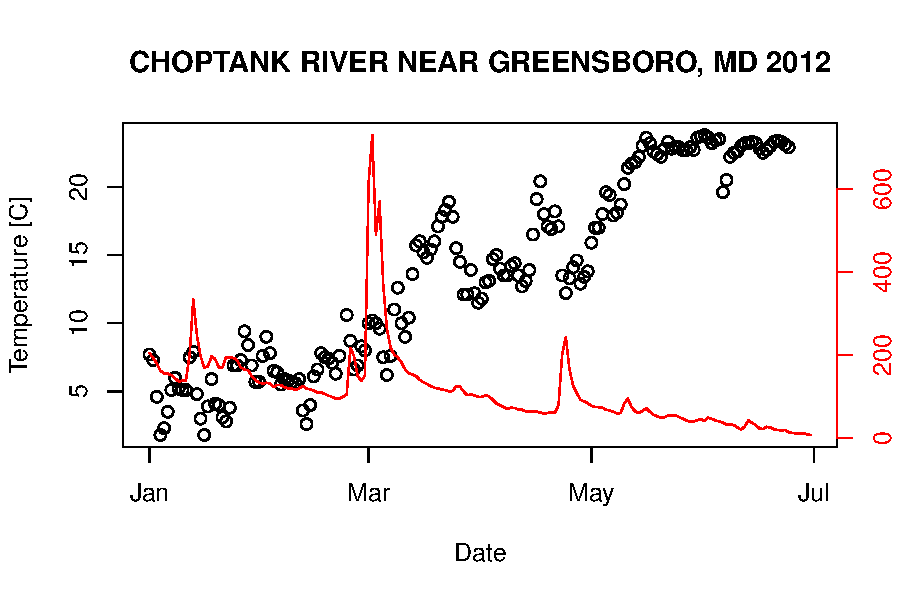
\includegraphics{dataRetrieval-fig1}
\end{center}
\caption{Temperature and discharge plot of Choptank River in 2012.}
\label{fig:TD}
\end{figure}


There are occasions where NWIS values are not reported as numbers, instead there might be text describing a certain event such as \texttt{"}Ice\texttt{"}.  Any value that cannot be converted to a number will be reported as NA in this package.

\FloatBarrier
%------------------------------------------------------------
\subsection{Unit Values}
\label{sec:usgsRT}
%------------------------------------------------------------
Any data that are collected at regular time intervals (such as 15-minute or hourly) are known as \texttt{"}Unit Values\texttt{"} - many of these are delivered on a real time basis and very recent data (even less than an hour old in many cases) are available through the function retrieveUnitNWISData.  Some of these Unit Values are available for the past several years, and some are only available for a recent time period such as 120 days or a year.  Here is an example of a retrieval of such data.  

\begin{Schunk}
\begin{Sinput}
> parameterCd <- "00060"  # Discharge (cfs)
> startDate <- "2012-05-12" 
> # or use (yesterday): startDate <- as.character(Sys.Date()-1)
> endDate <- "2012-05-13" 
> # or use (today):  endDate <- as.character(Sys.Date())
> dischargeToday <- retrieveUnitNWISData(siteNumber, parameterCd, 
         startDate, endDate)
\end{Sinput}
\end{Schunk}
Which produces the following dataframe:
\begin{Schunk}
\begin{Soutput}
  agency     site            dateTime X02_00060_00011 X02_00060_00011_cd
1   USGS 01491000 2012-05-12 00:00:00              83                  A
2   USGS 01491000 2012-05-12 00:15:00              83                  A
3   USGS 01491000 2012-05-12 00:30:00              83                  A
4   USGS 01491000 2012-05-12 00:45:00              83                  A
5   USGS 01491000 2012-05-12 01:00:00              85                  A
6   USGS 01491000 2012-05-12 01:15:00              83                  A
\end{Soutput}
\end{Schunk}

Note that time now becomes important, so the variable datetime is a POSIXct, and the time zone is included in a separate column. Data is pulled from \url{http://waterservices.usgs.gov/rest/IV-Test-Tool.html}. There are occasions where NWIS values are not reported as numbers, instead a common example is \texttt{"}Ice\texttt{"}.  Any value that cannot be converted to a number will be reported as NA in this package.

A simple plotting example is shown in Figure \ref{fig:RT}:
\begin{Schunk}
\begin{Sinput}
> colnames <- names(dischargeToday)
> with(dischargeToday, plot(
   get(colnames[3]), get(colnames[4]),
   ylab="Discharge [cfs]",xlab=""
   ))
> title(ChoptankInfo$station.nm)
> 
\end{Sinput}
\end{Schunk}
\newpage

\begin{figure}
\begin{center}
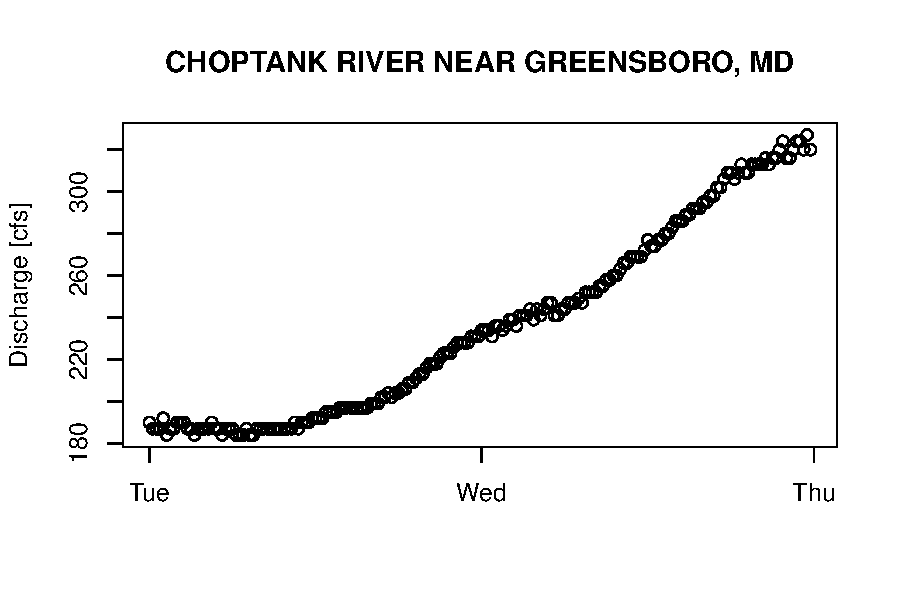
\includegraphics{dataRetrieval-fig2}
\end{center}
\caption{Real-time discharge plot of Choptank River from May 12-13, 2012.}
\label{fig:RT}
\end{figure}

\FloatBarrier
%------------------------------------------------------------
\subsection{Water Quality Values}
\label{sec:usgsWQP}
%------------------------------------------------------------
To get USGS water quality data from water samples collected at the streamgage (as distinct from unit values collected through some type of automatic monitor) we can use the Water Quality Data Portal: \url{http://www.waterqualitydata.us/}. The raw data are obtained from the function  getRawQWData, with the similar input arguments: siteNumber, parameterCd, startDate, endDate, and interactive. The difference is in parameterCd, in this function multiple parameters can be queried using a \texttt{"};\texttt{"} separator, and setting parameterCd to \texttt{"}\texttt{"} will return all of the measured observations. The raw data can be overwelming (see Appendix \ref{sec:appendix2WQP}), a simplified version of the data can be obtained using getQWData.There is a large amount of data returned for each observation. 


\begin{Schunk}
\begin{Sinput}
> # Dissolved Nitrate parameter codes:
> parameterCd <- c("00618","71851")
> startDate <- "1979-10-11"
> endDate <- "2012-12-18"
> dissolvedNitrate <- getRawQWData(siteNumber, parameterCd, 
       startDate, endDate)
> dissolvedNitrateSimple <- getQWData(siteNumber, parameterCd, 
         startDate, endDate)
> names(dissolvedNitrateSimple)
\end{Sinput}
\begin{Soutput}
[1] "dateTime"        "qualifier.00618" "value.00618"     "qualifier.71851"
[5] "value.71851"    
\end{Soutput}
\end{Schunk}
Note that in this dataframe, datetime is imported as Dates (no times are included), and the qualifier is either blank or \texttt{"}\verb@<@\texttt{"} signifying a censored value. A plotting example is shown in Figure \ref{fig:nitrate}.

\begin{Schunk}
\begin{Sinput}
> with(dissolvedNitrateSimple, plot(
   dateTime, value.00618,
   xlab="Date",ylab = paste(parameterINFO$srsname,
       "[",parameterINFO$parameter_units,"]")
   ))
> title(ChoptankInfo$station.nm)
\end{Sinput}
\end{Schunk}

\begin{figure}
\begin{center}
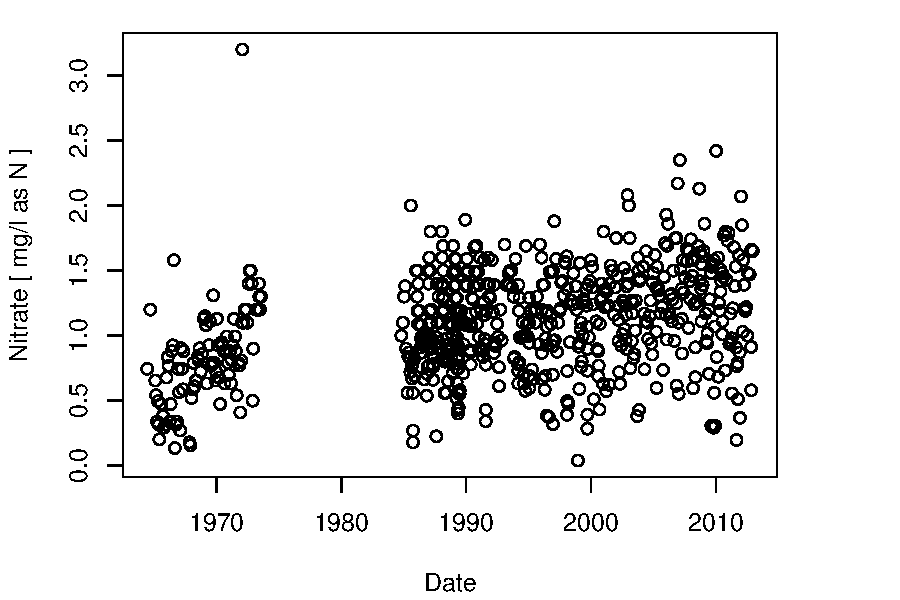
\includegraphics{dataRetrieval-fig3}
\end{center}
\caption{Nitrate plot of Choptank River.}
\label{fig:nitrate}
\end{figure}

\FloatBarrier
%------------------------------------------------------------
\subsection{STORET Water Quality Retrievals}
\label{sec:usgsSTORET}
%------------------------------------------------------------
There are additional data sets available on the Water Quality Data Portal (\url{http://www.waterqualitydata.us/}).  These data sets can be housed in either the STORET (data from EPA) or NWIS database.  Since STORET does not use USGS parameter codes, a \texttt{"}characteristic name\texttt{"} must be supplied.  The following example retrieves specific conductance from a DNR site in Wisconsin.

\begin{Schunk}
\begin{Sinput}
> specificCond <- getWQPData('WIDNR_WQX-10032762', 
         'Specific conductance', '', '')
> head(specificCond)
\end{Sinput}
\begin{Soutput}
    dateTime qualifier.Specific conductance value.Specific conductance
1 2011-02-14                                                      1360
2 2011-02-17                                                      1930
3 2011-03-03                                                      1240
4 2011-03-10                                                      1480
5 2011-03-29                                                      1130
6 2011-04-07                                                      1200
\end{Soutput}
\end{Schunk}

\FloatBarrier
%------------------------------------------------------------
\subsection{URL Construction}
\label{sec:usgsURL}
%------------------------------------------------------------
There may be times when you might be interested in seeing the URL (web address) that was used to obtain the raw data. The constructNWISURL function returns the URL.  Aside from input variables that have already been described, there is a new argument \texttt{"}service\texttt{"}. The service argument can be \texttt{"}dv\texttt{"} (daily values), \texttt{"}uv\texttt{"} (unit values), \texttt{"}qw\texttt{"} (NWIS water quality values), or \texttt{"}wqp\texttt{"} (general Water Quality Portal values).
 

\begin{Schunk}
\begin{Sinput}
> # Dissolved Nitrate parameter codes:
> pCode <- c("00618","71851")
> startDate <- "1964-06-11"
> endDate <- "2012-12-18"
> url_qw <- constructNWISURL(siteNumber,pCode,startDate,endDate,'qw')
> url_dv <- constructNWISURL(siteNumber,"00060",startDate,endDate,'dv',statCd="00003")
> url_uv <- constructNWISURL(siteNumber,"00060",startDate,endDate,'uv')
\end{Sinput}
\end{Schunk}

\FloatBarrier
%------------------------------------------------------------
\section{Data Retrievals Structured For Use In The EGRET Package}
%------------------------------------------------------------ 
Rather than using the raw data as retrieved by the web, the dataRetrieval package also includes functions that return the data in a structure that has been designed to work with the EGRET R package (\url{https://github.com/USGS-R/EGRET/wiki}). In general, these dataframes may be much more 'R-friendly' than the raw data, and will contain additional date information that allows for efficient data analysis.

In this section, we use 3 dataRetrieval functions to get sufficient data to perform an EGRET analysis.  We will continue analyzing the Choptank River. We will be retrieving essentially the same data that were retrieved in the previous section, but in this case it will be structured into three EGRET-specific dataframes.  The daily discharge data will be placed in a dataframe called Daily.  The nitrate sample data will be placed in a dataframe called Sample.  The data about the site and the parameter will be placed in a dataframe called INFO.  Although these dataframes were designed to work with the EGRET R package, they can be very useful for a wide range of hydrologic studies that don't use EGRET.

%------------------------------------------------------------
\subsection{INFO Data}
%------------------------------------------------------------
The function to obtain metadata, or data about the streamgage and measured parameters is getMetaData. This function combines getSiteFileData and getParameterInfo, producing one dataframe called INFO.

\begin{Schunk}
\begin{Sinput}
> parameterCd <- "00618"
> INFO <-getMetaData(siteNumber,parameterCd, interactive=FALSE)
\end{Sinput}
\end{Schunk}

Column names in the INFO dataframe are listed in Appendix 2 (\ref{sec:appendix2INFO}).

\FloatBarrier
%------------------------------------------------------------
\subsection{Daily Data}
%------------------------------------------------------------
The function to obtain the daily values (discharge in this case) is getDVData.  It requires the inputs siteNumber, ParameterCd, StartDate, EndDate, interactive, and convert. Most of these arguments are described in the previous section, however \texttt{"}convert\texttt{"} is a new argument (defaults to TRUE), and it tells the program to convert the values from cubic feet per second (cfs) to cubic meters per second (cms). For EGRET applications with NWIS web retrieval, do not use this argument (the default is TRUE), EGRET assumes that discharge is always in cubic meters per second. If you don't want this conversion and are not using EGRET, set convert=FALSE in the function call. 

\begin{Schunk}
\begin{Sinput}
> siteNumber <- "01491000"
> startDate <- "2000-01-01"
> endDate <- "2013-01-01"
> # This call will get NWIS data that is in cfs, and convert it
> # to cms since we didn't override the default in the convert argument:
> Daily <- getDVData(siteNumber, "00060", startDate, endDate,interactive=FALSE)
\end{Sinput}
\end{Schunk}

Details of the Daily dataframe are listed below:

% latex table generated in R 3.0.0 by xtable 1.7-1 package
% Mon Apr 08 10:09:57 2013
\begin{tabular}{llll}
  \hline
ColumnName & Type & Description & Units \\ 
  \hline
Date & Date & Date & date \\ 
  Q & number & Discharge & cms \\ 
  Julian & number & Number of days since January 1, 1850 & days \\ 
  Month & integer & Month of the year [1-12] & months \\ 
  Day & integer & Day of the year [1-366] & days \\ 
  DecYear & number & Decimal year & years \\ 
  MonthSeq & integer & Number of months since January 1, 1850 & months \\ 
  Qualifier & string & Qualifing code & character \\ 
  i & integer & Index of days from the start of the data frame & days \\ 
  LogQ & number & Natural logarithm of Q & numeric \\ 
  Q7 & number & 7 day running average of Q & cms \\ 
  Q30 & number & 30 running average of Q & cms \\ 
   \hline
\end{tabular}\\*

If there are discharge values of zero, the code will add a small constant to all of the daily discharges.  This constant is 0.001 times the mean discharge.  The code will also report on the number of zero values and the size of the constant.  EGRET should only be used if the number of zero values is a very small fraction of the total days in the record (say less than 0.1\% of the days).  Columns Q7 and Q30 are the 7 and 30 day running averages for the 7 or 30 days ending on this specific date.

\FloatBarrier
%------------------------------------------------------------
\subsection{Sample Data}
%------------------------------------------------------------
The function to obtain sample data from the water quality portal is getSampleData. The arguments for this function are also siteNumber, ParameterCd, StartDate, EndDate, interactive. These are the same inputs as getRawQWData or getQWData as described in the previous section.

\begin{Schunk}
\begin{Sinput}
> Sample <-getSampleData(siteNumber,parameterCd,
       startDate, endDate,interactive=FALSE)
\end{Sinput}
\end{Schunk}

Details of the Sample dataframe are listed below:

% latex table generated in R 3.0.0 by xtable 1.7-1 package
% Mon Apr 08 10:09:58 2013
\begin{table}[!ht]
\centering
\caption{Sample dataframe} 
\begin{tabular}{llll}
  \hline
ColumnName & Type & Description & Units \\ 
  \hline
Date & Date & Date & date \\ 
  ConcLow & number & Lower limit of concentration & mg/L \\ 
  ConcHigh & number & Upper limit of concentration & mg/L \\ 
  Uncen & integer & Uncensored data (1=true, 0=false) & integer \\ 
  ConcAve & number & Average of ConcLow and ConcHigh & mg/L \\ 
  Julian & number & Number of days since January 1, 1850 & days \\ 
  Month & integer & Month of the year [1-12] & months \\ 
  Day & integer & Day of the year [1-366] & days \\ 
  DecYear & number & Decimal year & years \\ 
  MonthSeq & integer & Number of months since January 1, 1850 & months \\ 
  SinDY & number & Sine of DecYear & numeric \\ 
  CosDY & number & Cosine of DecYear & numeric \\ 
  Q \footnotemark[1] & number & Discharge & cms \\ 
  LogQ \footnotemark[1] & number & Natural logarithm of flow & numeric \\ 
   \hline
\end{tabular}
\end{table}\footnotetext[1]{Flow columns are populated from data in the Daily dataframe after calling the mergeReport function.}

\FloatBarrier
%------------------------------------------------------------
\subsection{Censored Values: Summation Explanation}
%------------------------------------------------------------
In the typical case where none of the data are censored (that is, no values are reported as \texttt{"}less-than\texttt{"} values) the ConcLow = ConcHigh = ConcAve all of which are equal to the reported value and Uncen=0.  In the typical form of censoring where a value is reported as less than the reporting limit, then ConcLow = NA, ConcHigh = reporting limit, ConcAve = 0.5 * reporting limit, and Uncen = 1.

As an example to understand how the dataRetrieval package handles a more complex censoring problem, let us say that in 2004 and earlier, we computed a total phosphorus (tp) as the sum of dissolved phosphorus (dp) and particulate phosphorus (pp). From 2005 and onward, we have direct measurements of total phosphorus (tp). A small subset of this fictional data looks like this:

\begin{center}

% latex table generated in R 3.0.0 by xtable 1.7-1 package
% Mon Apr 08 10:09:58 2013
\begin{tabular}{llrlrlr}
  \hline
cdate & rdp & dp & rpp & pp & rtp & tp \\ 
  \hline
2003-02-15 &  & 0.02 &  & 0.50 &  &  \\ 
  2003-06-30 & $<$ & 0.01 &  & 0.30 &  &  \\ 
  2004-09-15 & $<$ & 0.00 & $<$ & 0.20 &  &  \\ 
  2005-01-30 &  &  &  &  &  & 0.43 \\ 
  2005-05-30 &  &  &  &  & $<$ & 0.05 \\ 
  2005-10-30 &  &  &  &  & $<$ & 0.02 \\ 
   \hline
\end{tabular}
\end{center}


The dataRetrieval package will \texttt{"}add up\texttt{"} all the values in a given row to form the total for that sample. Thus, you only want to enter data that should be added together. For example, we might know the value for dp on 5/30/2005, but we don't want to put it in the table because under the rules of this data set, we are not suppose to add it in to the values in 2005.

For every sample, the EGRET package requires a pair of numbers to define an interval in which the true value lies (ConcLow and ConcHigh). In a simple non-censored case (the reported value is above the detection limit), ConcLow equals ConcHigh and the interval collapses down to a single point.In a simple censored case, the value might be reported as <0.2, then ConcLow=NA and ConcHigh=0.2. We use NA instead of 0 as a way to elegantly handle future logarithm calculations.

For the more complex example case, let us say dp is reported as <0.01 and pp is reported as 0.3. We know that the total must be at least 0.3 and could be as much as 0.31. Therefore, ConcLow=0.3 and ConcHigh=0.31. Another case would be if dp is reported as <0.005 and pp is reported <0.2. We know in this case that the true value could be as low as zero, but could be as high as 0.205. Therefore, in this case, ConcLow=NA and ConcHigh=0.205. The Sample dataframe for the example data is therefore:

\begin{Schunk}
\begin{Soutput}
        Date ConcLow ConcHigh Uncen ConcAve Julian Month Day  DecYear MonthSeq
1 2003-02-15   0.520    0.520     1   0.520  55927     2  46 2003.124     1838
2 2003-06-30   0.310    0.310     1   0.310  56062     6 181 2003.493     1842
3 2004-09-15   0.205    0.205     1   0.205  56505     9 259 2004.706     1857
4 2005-01-30   0.430    0.430     1   0.430  56642     1  30 2005.081     1861
5 2005-05-30   0.050    0.050     1   0.050  56762     5 150 2005.408     1865
6 2005-10-30   0.020    0.020     1   0.020  56915    10 303 2005.827     1870
        SinDY      CosDY
1  0.70406552  0.7101350
2  0.04290476 -0.9990792
3 -0.96251346 -0.2712339
4  0.48505985  0.8744810
5  0.54391895 -0.8391378
6 -0.88668032  0.4623830
\end{Soutput}
\end{Schunk}

\FloatBarrier
%------------------------------------------------------------ 
\subsection{User-Generated Data Files}
%------------------------------------------------------------ 
Aside from retrieving data from the USGS web services, the dataRetrieval package includes functions to generate the Daily and Sample data frame from local files.

%------------------------------------------------------------ 
\subsubsection{getDailyDataFromFile}
%------------------------------------------------------------ 
getDailyDataFromFile will load a user-supplied text file and convert it to the Daily dataframe. The file should have two columns, the first dates, the second values.  The dates should be formatted either mm/dd/yyyy or yyyy-mm-dd. Using a 4-digit year is required. This function has the following inputs: filePath, fileName,hasHeader (TRUE/FALSE), separator, qUnit, and interactive (TRUE/FALSE). filePath is a string that defines the path to your file. This can either be a full path, or path relative to your R working directory. The input fileName is a string that defines the file name (including the extension).

Text files that contain this sort of data require some sort of a separator, for example, a 'csv' file (comma-separated value) file uses a comma to separate the date and value column. A tab delimited file would use a tab (\texttt{"}\verb@\t@\texttt{"}) rather than the comma (\texttt{"},\texttt{"}). The type of separator you use can be defined in the function call in the \texttt{"}separator\texttt{"} argument, the default is \texttt{"},\texttt{\texttt{"}}. Another function input is a logical variable: hasHeader.  The default is TRUE. If your data does not have column names, set this variable to FALSE.

Finally, qUnit is a numeric argument that defines the discharge units used in the input file.  The default is qUnit = 1 which assumes discharge is in cubic feet per second.  If the discharge in the file is already in cubic meters per second then set qUnit = 2.  If it is in some other units (like liters per second or acre-feet per day), the user will have to pre-process the data with a unit conversion that changes it to either cubic feet per second or cubic meters per second.

So, if you have a file called \texttt{"}ChoptankRiverFlow.txt\texttt{"} located in a folder called \texttt{"}RData\texttt{"} on the C drive (this is a Window's example), and the file is structured as follows (tab-separated):
\begin{verbatim}
date  Qdaily
10/1/1999  107
10/2/1999	85
10/3/1999	76
10/4/1999	76
10/5/1999	113
10/6/1999	98
...
\end{verbatim}

The call to open this file, convert the flow to cubic meters per second, and populate the Daily data frame would be:
\begin{Schunk}
\begin{Sinput}
> fileName <- "ChoptankRiverFlow.txt"
> filePath <-  "C:/RData/"
> Daily <- getDailyDataFromFile(filePath,fileName,separator="\t",interactive=FALSE)
\end{Sinput}
\end{Schunk}

\FloatBarrier
%------------------------------------------------------------ 
\subsubsection{getSampleDataFromFile}
%------------------------------------------------------------ 
Similarly to the previous section, getSampleDataFromFile will import a user-generated file and populate the Sample dataframe. The difference between sample data and flow data is that the code requires a third column that contains a remark code, either blank or \texttt{"}\verb@<@\texttt{"}, which will tell the program that the data was 'left-censored' (or, below the detection limit of the sensor). Therefore, the data is required to be in the form: date, remark, value.  If multiple constituents are going to be used, the format can be date, remark\_A, value\_A, remark\_b, value\_b, etc... An example of a comma-delimited file would be:

\begin{verbatim}
cdate;remarkCode;Nitrate
10/7/1999,,1.4
11/4/1999,<,0.99
12/3/1999,,1.42
1/4/2000,,1.59
2/3/2000,,1.54
...
\end{verbatim}
The call to open this file, and populate the Sample dataframe would be:
\begin{Schunk}
\begin{Sinput}
> fileName <- "ChoptankRiverNitrate.csv"
> filePath <-  "C:/RData/"
> Sample <- getSampleDataFromFile(filePath,fileName,separator=",",interactive=FALSE)
\end{Sinput}
\end{Schunk}

\FloatBarrier
%------------------------------------------------------------
\subsection{Merge Report}
%------------------------------------------------------------
Finally, there is a function called mergeReport that will look at both the Daily and Sample dataframe, and populate Q and LogQ columns into the Sample dataframe. The default arguments are Daily and Sample, however if you want to use other similarly structured dataframes, you can specify localDaily or localSample. Once mergeReport has been run, the Sample dataframe will be augumented with the daily discharges for all the days with samples.  None of the water quality functions in EGRET will work without first having run the mergeReport function.


\begin{Schunk}
\begin{Sinput}
> siteNumber <- "01491000"
> parameterCd <- "00631"  # Nitrate
> startDate <- "2000-01-01"
> endDate <- "2013-01-01"
> Daily <- getDVData(siteNumber, "00060", startDate, endDate,interactive=FALSE)
> Sample <- getSampleData(siteNumber,parameterCd, startDate, endDate, interactive=FALSE)
> Sample <- mergeReport()
\end{Sinput}
\begin{Soutput}
 Discharge Record is 4750 days long, which is 13 years
 First day of the discharge record is 2000-01-01 and last day is 2013-01-01
 The water quality record has 220 samples
 The first sample is from 2000-01-04 and the last sample is from 2012-12-18
 Discharge: Minimum, mean and maximum 0.00991 4.55 246
 Concentration: Minimum, mean and maximum 0.2 1.3 2.4
 Percentage of the sample values that are censored is 0 %
\end{Soutput}
\begin{Sinput}
> head(Sample)
\end{Sinput}
\begin{Soutput}
        Date ConcLow ConcHigh Uncen ConcAve Julian Month Day  DecYear MonthSeq
1 2000-01-04    1.59     1.59     1    1.59  54789     1   4 2000.010     1801
2 2000-02-03    1.54     1.54     1    1.54  54819     2  34 2000.092     1802
3 2000-02-15    1.37     1.37     1    1.37  54831     2  46 2000.124     1802
4 2000-02-19    1.24     1.24     1    1.24  54835     2  50 2000.135     1802
5 2000-03-23    0.52     0.52     1    0.52  54868     3  83 2000.225     1803
6 2000-06-05    1.11     1.11     1    1.11  54942     6 157 2000.428     1806
       SinDY      CosDY         Q      LogQ
1 0.06004896  0.9981954  2.746734 1.0104126
2 0.54391895  0.8391378  3.936042 1.3701756
3 0.70406552  0.7101350 10.845352 2.3837366
4 0.75113193  0.6601521 15.517632 2.7419769
5 0.98808790  0.1538906 56.916861 4.0415916
6 0.43939951 -0.8982918  1.812278 0.5945847
\end{Soutput}
\end{Schunk}

\FloatBarrier
%------------------------------------------------------------
\subsection{EGRET Plots}
%------------------------------------------------------------
As has been mentioned, the data is specifically formatted to be used with the EGRET package. The EGRET package has powerful modeling capabilities using WRTDS, but also has a variety of graphing and tablular tools to explore the data without using the WRTDS algorithm. See the EGRET vignette, user guide, and/or wiki (\url{https://github.com/USGS-R/EGRET/wiki}) for detailed information. The following figure is an example of one of the plotting functions that can be used directly from the dataRetrieval dataframes.

\begin{Schunk}
\begin{Sinput}
> # Continuing Choptank example from the previous sections
> library(EGRET)
> multiPlotDataOverview()
\end{Sinput}
\end{Schunk}

\begin{figure}[ht]
\begin{center}

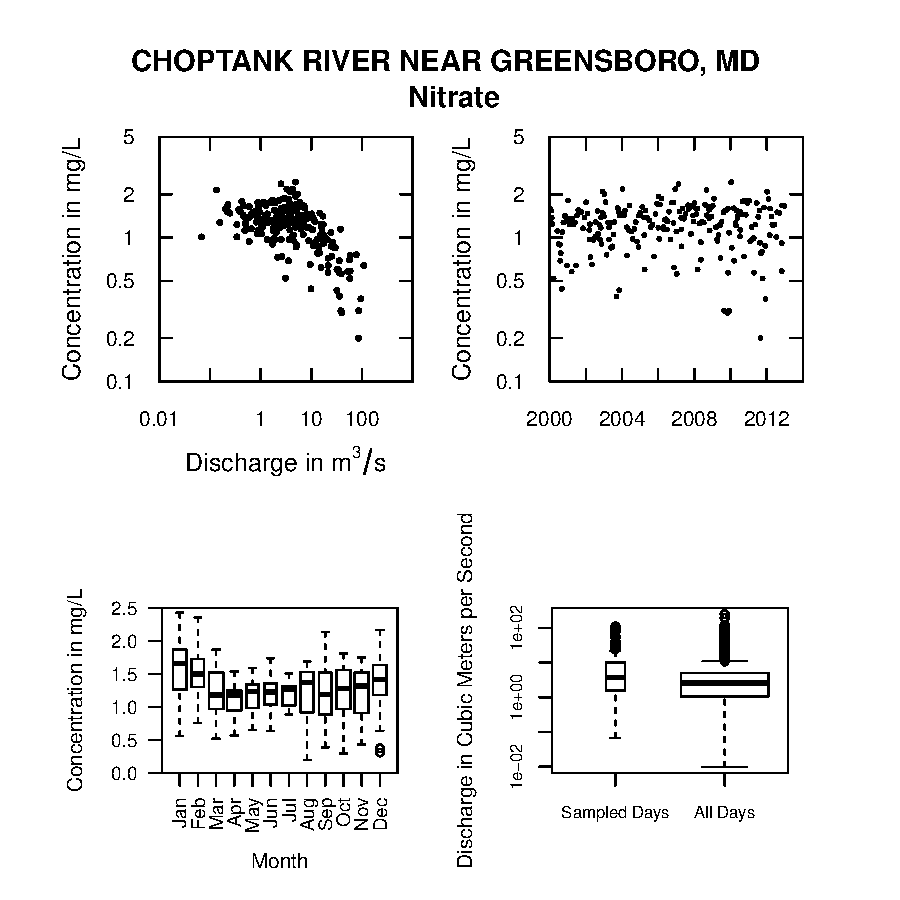
\includegraphics{dataRetrieval-figegretEx}
\end{center}
\caption{Default multiPlotDataOverview}
\label{fig:multiPlotDataOverview}
\end{figure}

\clearpage
\appendix
%------------------------------------------------------------ 
\section{Getting Started in R}
\label{sec:appendix1}
%------------------------------------------------------------ 
This section describes the options for downloading and installing the dataRetrieval package.

%------------------------------------------------------------
\subsection{New to R?}
%------------------------------------------------------------ 
If you are new to R, you will need to first install the latest version of R, which can be found here: \url{http://www.r-project.org/}.

There are many options for running and editing R code, one nice environment to learn R is RStudio. RStudio can be downloaded here: \url{http://rstudio.org/}. Once R and RStudio are installed, the dataRetrieval package needs to be installed as described in the next section.

At any time, you can get information about any function in R by typing a question mark before the functions name.  This will open a file (in RStudio, in the Help window) that describes the function, the required arguments, and provides working examples.

\begin{Schunk}
\begin{Sinput}
> ?removeDuplicates
\end{Sinput}
\end{Schunk}

To see the raw code for a particular code, type the name of the function:
\begin{Schunk}
\begin{Sinput}
> removeDuplicates
\end{Sinput}
\begin{Soutput}
function (localSample = Sample) 
{
    Sample1 <- localSample[!duplicated(localSample[c("DecYear", 
        "ConcHigh")]), ]
    return(Sample1)
}
<environment: namespace:dataRetrieval>
\end{Soutput}
\end{Schunk}


%------------------------------------------------------------
\subsection{R User: Installing dataRetrieval}
%------------------------------------------------------------ 
Before installing dataRetrieval, the zoo packages must be installed from CRAN:

\begin{Schunk}
\begin{Sinput}
> install.packages("zoo")
> install.packages("dataRetrieval", repos="http://usgs-r.github.com", type="source")
\end{Sinput}
\end{Schunk}

It is a good idea to re-start the R enviornment after installing the package, especially if installing an updated version. Some users have found it necessary to delete the previous version's package folder before installing newer version of dataRetrieval. If you are experiencing issues after updating a package, trying deleting the package folder - the default location for Windows is something like this: C:/Users/userA/Documents/R/win-library/2.15/dataRetrieval, and the default for a Mac: /Users/userA/Library/R/2.15/library/dataRetrieval. Then, re-install the package using the directions above. Moving to CRAN should solve this problem.

After installing the package, you need to open the library each time you re-start R.  This is done with the simple command:
\begin{Schunk}
\begin{Sinput}
> library(dataRetrieval)
\end{Sinput}
\end{Schunk}
Using RStudio, you could alternatively click on the checkbox for dataRetrieval in the Packages window.

%------------------------------------------------------------
\subsection{R Developers: Installing dataRetrieval from gitHub}
%------------------------------------------------------------
Alternatively, R-developers can install the latest working version of dataRetrieval directly from gitHub using the devtools package (available on CRAN).  Rtools (for Windows) and appropriate \LaTeX\ tools are required. Be aware that the version installed using this method isn't necessarily the same as the version in the stable release branch.  


\begin{Schunk}
\begin{Sinput}
> library(devtools)
> install_github("dataRetrieval", "USGS-R")
\end{Sinput}
\end{Schunk}
To then open the library, simply type:

\begin{Schunk}
\begin{Sinput}
> library(dataRetrieval)
\end{Sinput}
\end{Schunk}

%------------------------------------------------------------ 
\section{Columns Names}
\label{sec:appendix2}
%------------------------------------------------------------ 

%------------------------------------------------------------
\subsection{INFO dataframe}
\label{sec:appendix2INFO}
%------------------------------------------------------------

% latex table generated in R 3.0.0 by xtable 1.7-1 package
% Mon Apr 08 10:10:02 2013
\begin{tabular}{l}
  \hline
  \hline
agency.cd \\ 
  site.no \\ 
  station.nm \\ 
  site.tp.cd \\ 
  lat.va \\ 
  long.va \\ 
  dec.lat.va \\ 
  dec.long.va \\ 
  coord.meth.cd \\ 
  coord.acy.cd \\ 
  coord.datum.cd \\ 
  dec.coord.datum.cd \\ 
  district.cd \\ 
  state.cd \\ 
  county.cd \\ 
  country.cd \\ 
  map.nm \\ 
  map.scale.fc \\ 
  alt.va \\ 
  alt.meth.cd \\ 
  alt.acy.va \\ 
  alt.datum.cd \\ 
  huc.cd \\ 
  basin.cd \\ 
  topo.cd \\ 
  construction.dt \\ 
  inventory.dt \\ 
  drain.area.va \\ 
  contrib.drain.area.va \\ 
  tz.cd \\ 
  local.time.fg \\ 
  reliability.cd \\ 
  project.no \\ 
  queryTime \\ 
  drainSqKm \\ 
  shortName \\ 
  staAbbrev \\ 
  param.nm \\ 
  param.units \\ 
  paramShortName \\ 
  paramNumber \\ 
  constitAbbrev \\ 
   \hline
\end{tabular}
\FloatBarrier

%------------------------------------------------------------
\subsection{Water Quality Portal}
\label{sec:appendix2WQP}
%------------------------------------------------------------

There are 62 columns returned from the water quality portal. 

% latex table generated in R 3.0.0 by xtable 1.7-1 package
% Mon Apr 08 10:10:02 2013
\begin{tabular}{l}
  \hline
  \hline
OrganizationIdentifier \\ 
  OrganizationFormalName \\ 
  ActivityIdentifier \\ 
  ActivityTypeCode \\ 
  ActivityMediaName \\ 
  ActivityMediaSubdivisionName \\ 
  ActivityStartDate \\ 
  ActivityStartTime.Time \\ 
  ActivityStartTime.TimeZoneCode \\ 
  ActivityEndDate \\ 
  ActivityEndTime.Time \\ 
  ActivityEndTime.TimeZoneCode \\ 
  ActivityDepthHeightMeasure.MeasureValue \\ 
  ActivityDepthHeightMeasure.MeasureUnitCode \\ 
  ActivityDepthAltitudeReferencePointText \\ 
  ActivityTopDepthHeightMeasure.MeasureValue \\ 
  ActivityTopDepthHeightMeasure.MeasureUnitCode \\ 
  ActivityBottomDepthHeightMeasure.MeasureValue \\ 
  ActivityBottomDepthHeightMeasure.MeasureUnitCode \\ 
  ProjectIdentifier \\ 
  ActivityConductingOrganizationText \\ 
  MonitoringLocationIdentifier \\ 
  ActivityCommentText \\ 
  SampleAquifer \\ 
  HydrologicCondition \\ 
  HydrologicEvent \\ 
  SampleCollectionMethod.MethodIdentifier \\ 
  SampleCollectionMethod.MethodIdentifierContext \\ 
  SampleCollectionMethod.MethodName \\ 
  SampleCollectionEquipmentName \\ 
  ResultDetectionConditionText \\ 
  CharacteristicName \\ 
  ResultSampleFractionText \\ 
  ResultMeasureValue \\ 
  ResultMeasure.MeasureUnitCode \\ 
  MeasureQualifierCode \\ 
  ResultStatusIdentifier \\ 
  StatisticalBaseCode \\ 
  ResultValueTypeName \\ 
  ResultWeightBasisText \\ 
   \hline
\end{tabular}
\FloatBarrier

% latex table generated in R 3.0.0 by xtable 1.7-1 package
% Mon Apr 08 10:10:02 2013
\begin{tabular}{l}
  \hline
  \hline
ResultTimeBasisText \\ 
  ResultTemperatureBasisText \\ 
  ResultParticleSizeBasisText \\ 
  PrecisionValue \\ 
  ResultCommentText \\ 
  USGSPCode \\ 
  ResultDepthHeightMeasure.MeasureValue \\ 
  ResultDepthHeightMeasure.MeasureUnitCode \\ 
  ResultDepthAltitudeReferencePointText \\ 
  SubjectTaxonomicName \\ 
  SampleTissueAnatomyName \\ 
  ResultAnalyticalMethod.MethodIdentifier \\ 
  ResultAnalyticalMethod.MethodIdentifierContext \\ 
  ResultAnalyticalMethod.MethodName \\ 
  MethodDescriptionText \\ 
  LaboratoryName \\ 
  AnalysisStartDate \\ 
  ResultLaboratoryCommentText \\ 
  DetectionQuantitationLimitTypeName \\ 
  DetectionQuantitationLimitMeasure.MeasureValue \\ 
  DetectionQuantitationLimitMeasure.MeasureUnitCode \\ 
  PreparationStartDate \\ 
   \hline
\end{tabular}
\clearpage

%------------------------------------------------------------ 
\section{Creating tables in Microsoft from R}
\label{app:createWordTable}
%------------------------------------------------------------
There are a few steps that are required in order to create a table in a Microsoft product (Excel, Word, Powerpoint, etc.) from an R dataframe. There are certainly a variety of good methods, one of which is detailed here. The example we will step through here will be to create a table in Microsoft Word based on the dataframe tableData:

\begin{Schunk}
\begin{Sinput}
> ChoptankAvailableData <- getDataAvailability(siteNumber)
> ChoptankDailyData <- ChoptankAvailableData["dv" == ChoptankAvailableData$service,]
> ChoptankDailyData <- ChoptankDailyData["00003" == ChoptankDailyData$statCd,]
> pCodeINFO <- getMultipleParameterNames(ChoptankDailyData$parameter_cd, interactive=FALSE)
> ChoptankDailyData <- merge(ChoptankDailyData,pCodeINFO,by="parameter_cd")
> tableData <- with(ChoptankDailyData, 
       data.frame(
       shortName=srsname, 
       Start=startDate, 
       End=endDate, 
       Count=count,
       Units=parameter_units)
       )
\end{Sinput}
\end{Schunk}

First, save the dataframe as a tab delimited file (you don't want to use comma delimited because there are commas in some of the data elements):


\begin{Schunk}
\begin{Sinput}
> write.table(tableData, file="tableData.tsv",sep="\t",
             row.names = FALSE,quote=FALSE)
\end{Sinput}
\end{Schunk}

This will save a file in your working directory called tableData.tsv.  You can see your working directory by typing getwd() in the R console. Opening the file in a general-purpose text editor, you should see the following:

\begin{verbatim}
shortName  Start	End	Count	Units
Temperature, water	2010-10-01	2012-06-24	575	deg C
Stream flow, mean. daily	1948-01-01	2013-03-13	23814	cfs
Specific conductance	2010-10-01	2012-06-24	551	uS/cm @25C
Suspended sediment concentration (SSC)	1980-10-01	1991-09-30	3651	mg/l
Suspended sediment discharge	1980-10-01	1991-09-30	3652	tons/day
\end{verbatim}

To open this file in Excel:
\begin{enumerate}
\item Open Excel
\item Click on the File tab
\item Click on the Open option
\item Browse to the working directory (as shown in the results of getwd())
\item Next to the File name text box, change the dropdown type to All Files (*.*)
\item Double click tableData.tsv
\item A text import wizard will open up, in the first window, choose the Delimited radio button if it is not automatically picked, then click on Next.
\item In the second window, click on the Tab delimiter if it is not automatically checked, then click Finished.
\item Use the many formatting tools within Excel to customize the table
\end{enumerate}

From Excel, it is simple to copy and paste the tables in other Microsoft products. An example using one of the default Excel table formats is here.

\begin{figure}[ht!]
\centering
 \resizebox{0.9\textwidth}{!}{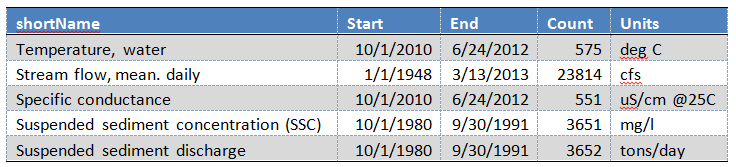
\includegraphics{table1.png}} 
\caption{A simple table produced in Microsoft Excel}
\label{overflow}
\end{figure}

\clearpage
%------------------------------------------------------------
% BIBLIO
%------------------------------------------------------------
\begin{thebibliography}{10}

\bibitem{HirschI}
Helsel, D.R. and R. M. Hirsch, 2002. Statistical Methods in Water Resources Techniques of Water Resources Investigations, Book 4, chapter A3. U.S. Geological Survey. 522 pages. \url{http://pubs.usgs.gov/twri/twri4a3/}

\bibitem{HirschII}
Hirsch, R. M., Moyer, D. L. and Archfield, S. A. (2010), Weighted Regressions on Time, Discharge, and Season (WRTDS), with an Application to Chesapeake Bay River Inputs. JAWRA Journal of the American Water Resources Association, 46: 857-880. doi: 10.1111/j.1752-1688.2010.00482.x \url{http://onlinelibrary.wiley.com/doi/10.1111/j.1752-1688.2010.00482.x/full}

\bibitem{HirschIII}
Sprague, L. A., Hirsch, R. M., and Aulenbach, B. T. (2011), Nitrate in the Mississippi River and Its Tributaries, 1980 to 2008: Are We Making Progress? Environmental Science \& Technology, 45 (17): 7209-7216. doi: 10.1021/es201221s \url{http://pubs.acs.org/doi/abs/10.1021/es201221s}

\end{thebibliography}

\end{document}

\end{document}
